\graphicspath{ {./root/4.Annex/1.AnnexAnnachiaraInspectionImages/} }

\subsubsection{Evaluator 2 inspection scores}

\begingroup
\setlength{\tabcolsep}{1.5cm}
\renewcommand{\arraystretch}{1.45}

\begin{small}

\rowcolors{2}{lightgray}{lightblue}
\begin{longtable}{l r}
	
	\hiderowcolors
	\textbf{Heuristic} & \textbf{Score} \\ \hline\\ 
	\showrowcolors
	 \endhead 
	
	H1. Visibility of system status & 2  \\
	H2. Match between system and the real world & 4  \\
	H3. User control and freedom & 2 \\
	H4. Consistency and standards & 1 \\
	H5. Error prevention & 3 \\
	H6. Recognition rather than recall & 4 \\
	H7. Flexibility and efficiency of use & 3 \\
	H8. Aesthetic and minimalist design & 1 \\
	H9. Help users recognize, diagnose and recover from errors & 4 \\
	H10. Help and documentation & 2 \\
	H11. Information overload & 2 \\
	H12. Consistency of page content structure  & 1 \\
	H13. Contextualized information & 2 \\
	H14. Content organisation (hierarchy) & 1 \\
	H15. Interaction consistency & 3 \\
	H16. Group navigation-1 & 2 \\
	H17. Group navigation-2 & 3 \\
	H18. Structural navigation & 3 \\
	H19. Semantic navigation & 3 \\
	H20. “Landmarks” & 3 \\
	H21. Text lay out & 3 \\
	H22. Interaction placeholders-semiotics & 3 \\
	H23. Interaction placeholders-consistency & 2 \\
	H24. Consistency of visual elements & 2 \\
	H25. Hierarchy-1 & 2 \\
	H26. Hierarchy-2 & 1 \\
	H27. Spatial allocation-1 & 4 \\
	H28. Spatial allocation-2 & 3 \\
	H29. Consistency of page spatial structure & 3 \\
	
\end{longtable}

\end{small}
\endgroup

\vspace{0.5cm}


\subsection*{Evaluator's comments}
\paragraph*{H1. Visibility of System Status - Score 2}
In general, the visibility of the system status is not respected when navigating the website, since the user is only informed about his/her current position is few pages and this can lead to confusion and frustration. 
Breadcrumbs are present only in few sections of the website and they and in the main menu the current position of the user is not highlighted (bold, underline etc...).

\begin{figure}[h]
	\centering
	\begin{center}
		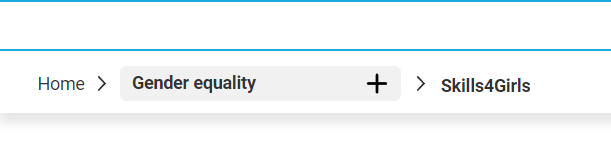
\includegraphics{Picture1.png}
	\end{center}
	\captionsetup{font=small}
	\caption{\textit{Breadcrumbs example.}}
	\label{fig:label1}
\end{figure}

\begin{figure}[h]
	\centering
	\begin{center}
		
\includegraphics[width=\textwidth]{Picture2.png}
	\end{center}
	\captionsetup{font=small}
	\caption{\textit{Main menu example.}}
	\label{fig:label2}
\end{figure}


\paragraph*{H2. Match Between the System and the Real World - Score 4}
In general, the language used in the website matches the users' existing knowledge and mental models, making it easy for the him/her to understand the information provided. The icons used in the website represent familiar concepts, facilitating the comprehension. 

\begin{figure}[h]
	\centering
	\begin{center}
		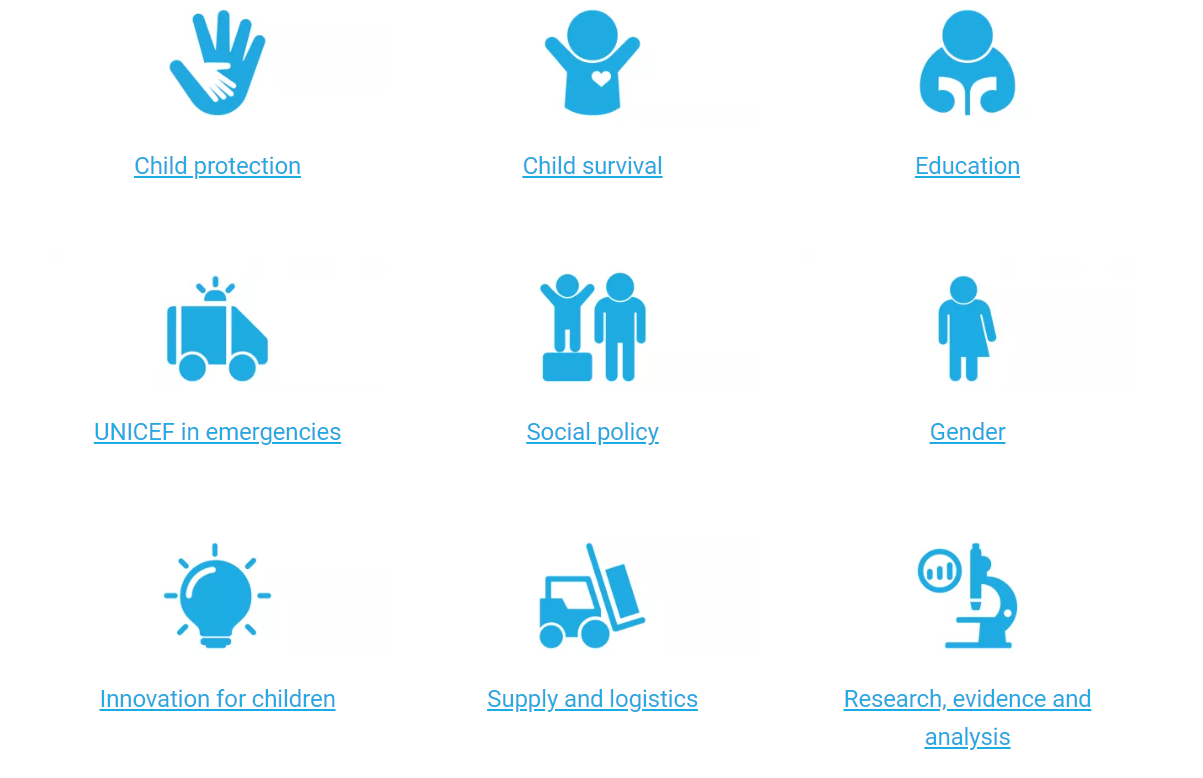
\includegraphics[width=0.6\textwidth]{Picture3.png}
	\end{center}
	\captionsetup{font=small}
	\caption{\textit{Icons representing familiar concepts.}}
	\label{fig:label3}
\end{figure}

\paragraph*{H3. User Control and Freedom - Score 2}
On the website you can always go back to the homepage by clicking on the logo in the upper left corner of the page or you can go back by using the navigational arrow. However, it can happen to be redirected to another website and in this case is not easy to understand how to go back to UNICEF Global, also because the pages that redirect to other website are not reported in different ways. When trying to go back from the page “Donate” the pop-up repeatedly shows up, making it difficult to exit the page and even frustrating. Moreover, the complexity of the website architecture making it hard for the user to have full control over the navigation.

\begin{figure}[h]
	\centering
	\begin{center}
		
\includegraphics[width=0.6\textwidth]{Picture4.png}
	\end{center}
	\captionsetup{font=small}
	\caption{\textit{UNICEF Global button.}}
	\label{fig:label4}
\end{figure}

\begin{figure}[h]
	\centering
	\begin{center}
		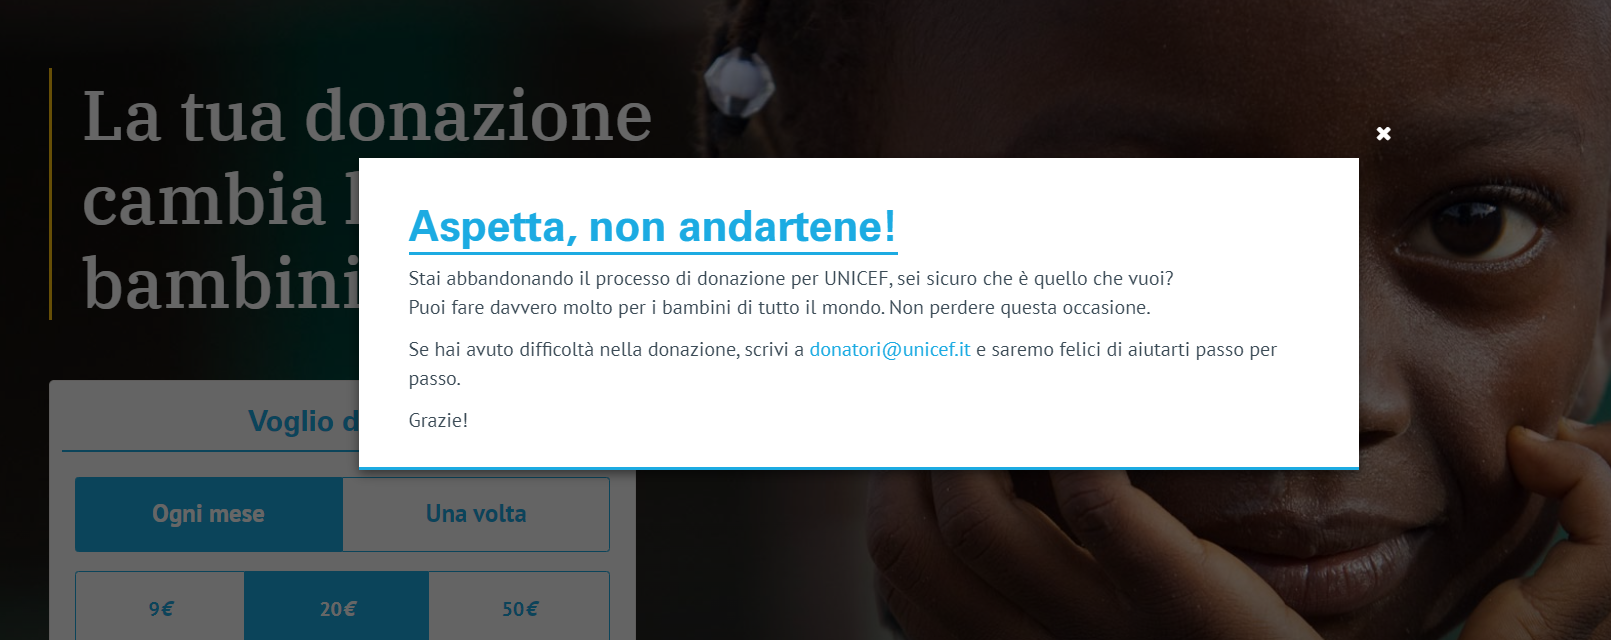
\includegraphics[width=0.6\textwidth]{Picture5.png}
	\end{center}
	\captionsetup{font=small}
	\caption{\textit{Donate page pop-up.}}
	\label{fig:label5}
\end{figure}

\paragraph*{H4. Consistency and Standars - Score 1}
The website partly follows the established industry conventions (external consistency) in terms of icons and for some aspects of the navigation (clicking on the logo brings to the homepage), but it totally lacks internal consistency. This compromises the learnability of the navigation, as well as resulting in increasing the users’ cognitive load. Moreover, the structure of the pages is always different in the positioning of the contents (text, call to action, links, images) making it necessary to understand several different patterns and forms of interactions for each screen.
There is a total lack of consistency of the buttons, for example the call to action for donating. In general, the buttons hardly follow a pattern of color, positioning and typography across the whole website.

\begin{figure}[h]
	\centering
	\begin{center}
		
\includegraphics[width=0.4\textwidth]{Picture6.png}
	\end{center}
	\captionsetup{font=small}
	\caption{\textit{Donate button example.}}
	\label{fig:label6}
\end{figure}

\begin{figure}[h]
	\centering
	\begin{center}
		
\includegraphics[width=0.4\textwidth]{Picture7.png}
	\end{center}
	\captionsetup{font=small}
	\caption{\textit{Different Donate button example.}}
	\label{fig:label7}
\end{figure}

Another example is that, despite being in the same section (What We Do), the pages “Covid-19 Response” and “Gender” follow to totally different organizations of the contents in the page and this inconsistency can be found across the whole website. The pages "Nutrition" and "Gender" present two different menu for the page navigation. In the main menu we can read the title "Gender", while the title of the page is "Gender equality", the same is for “All areas” that is the page “What we do”.
In addition, it is very complex to understand the differences between the cards, since a consistent design system is not used, and the hierarchy and disposition of the elements make it harder to have a clear and fast understanding of what the user can achieve by clicking on each card.
\\
\begin{figure}[h]
	\centering
	\begin{center}
		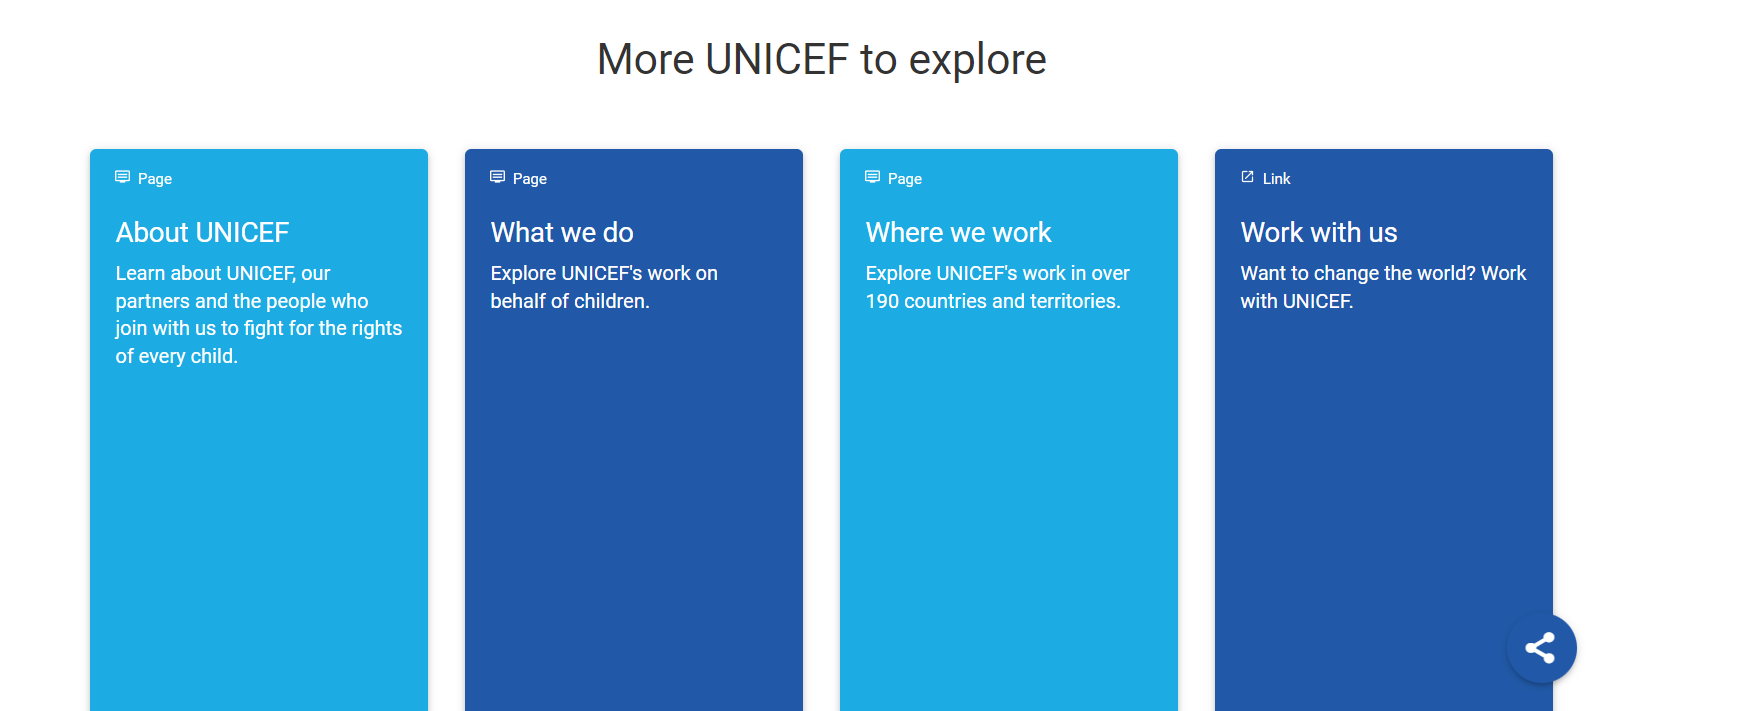
\includegraphics[width=0.6\textwidth]{Picture8.png}
	\end{center}
	\captionsetup{font=small}
	\caption{\textit{Card inconsistency 1.}}
	\label{fig:label8}
\end{figure}

\begin{figure}[h]
	\centering
	\begin{center}
		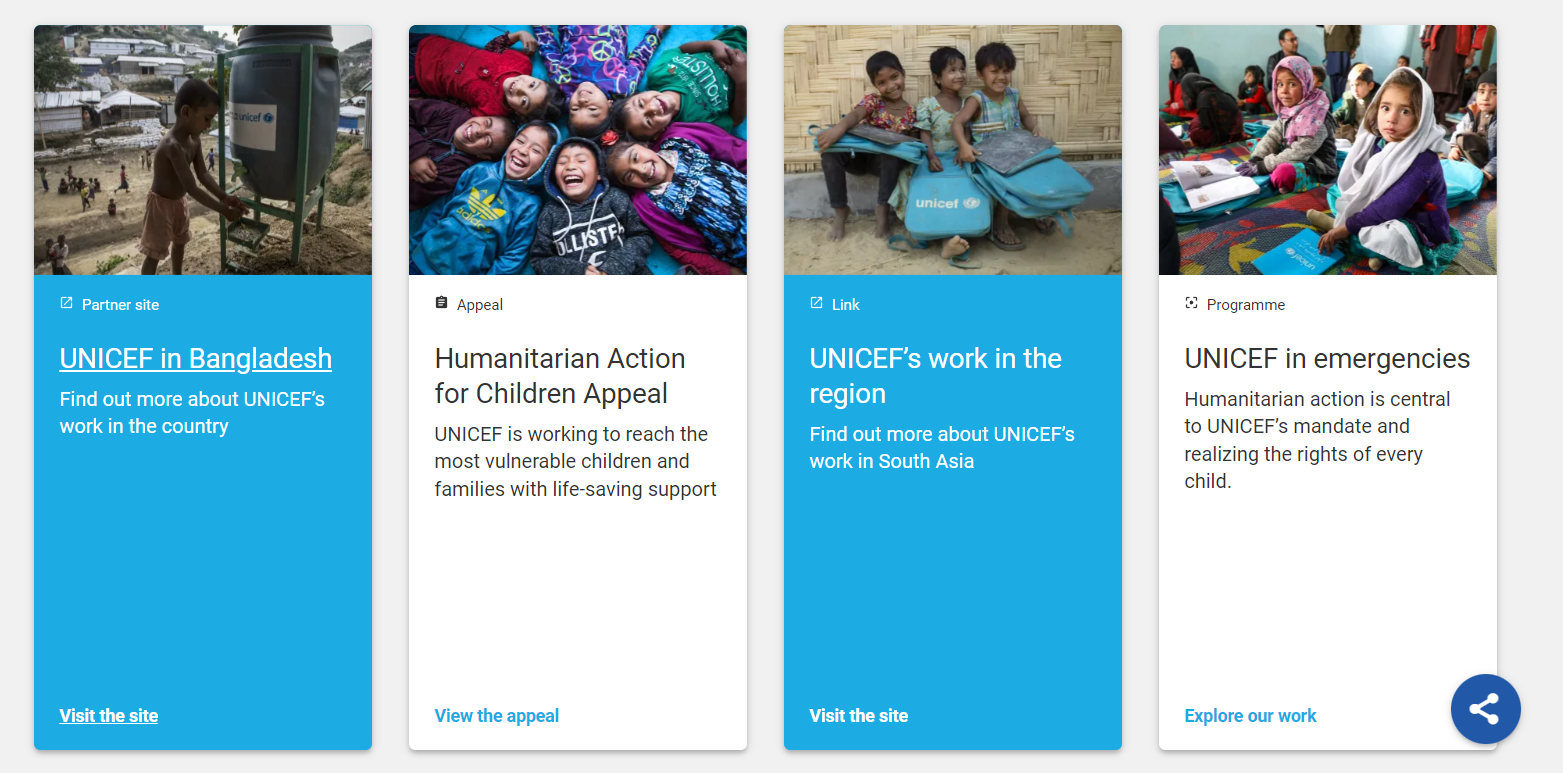
\includegraphics[width=0.6\textwidth]{Picture9.png}
	\end{center}
	\captionsetup{font=small}
	\caption{\textit{Card inconsistency 2.}}
	\label{fig:label9}
\end{figure}

\paragraph*{H5. Error Prevention - Score 3}
Due to the lack of consistency and the complexity of the website the navigation is not totally fluid, resulting in not preventing the user from making mistakes. The load of information present in each page contributes to increase the memory burden, mainly causing slips (right intent, wrong action). However, mistakes when filling forms are correctly highlighted, even though they are only reported after clicking “Submit”. 

\begin{figure}[h]
	\centering
	\begin{center}
		
\includegraphics[width=0.6\textwidth]{Picture10.png}
	\end{center}
	\captionsetup{font=small}
	\caption{\textit{Mistakes when filling forms in the “Contact” page.}}
	\label{fig:label10}
\end{figure}

\paragraph*{H6. Recognition rather than Recall - Score 4}
No major problems were found regarding this heuristic, since objects, actions, and options are usually visible across the website. For example, in the search field the suggestion makes it easier for the user to search for information.

\begin{figure}[h]
	\centering
	\begin{center}
		
\includegraphics[width=\textwidth]{Picture11.png}
	\end{center}
	\captionsetup{font=small}
	\caption{\textit{Suggestion.}}
	\label{fig:label11}
\end{figure}

\paragraph*{H7. Flexibility and Efficiency of Use - Score 3}
No customization or personalization is possible across the website and the interface is difficult to learn being very complex and full of information, making it hard for less experienced users to easily find the information needed. However, some shortcuts are present in the homepage, as well as in the “What We Do” page. Moreover, there is the possibility to adjust the contrast of the website with a landmark (same for changing language), but it does not change all the elements in the page.

\begin{figure}[h]
	\centering
	\begin{center}
		
\includegraphics[width=0.6\textwidth]{Picture11B.png}
	\end{center}
	\captionsetup{font=small}
	\caption{\textit{Change Language.}}
	\label{fig:label11B}
\end{figure}

\paragraph*{H8. Aesthetic and Minimalist Design - Score 1}
The interface is not simple or functional, as it is cluttered with many different design elements that often do not follow an established design system. In this way the interface is not supporting the users’ primary goals due to the overload of information. UNICEF website is complex, due to the need of presenting many different information that support and explain the cause, but its visual design is not focused on the essential and this tragically compromises the user experience.
For example, in the page "Better Mental Health" there is the possibility to take a quiz that fills the whole screen, despite being an unnecessary information. These kind of examples can be found in all pages across the whole website.

\begin{figure}[h]
	\centering
	\begin{center}
		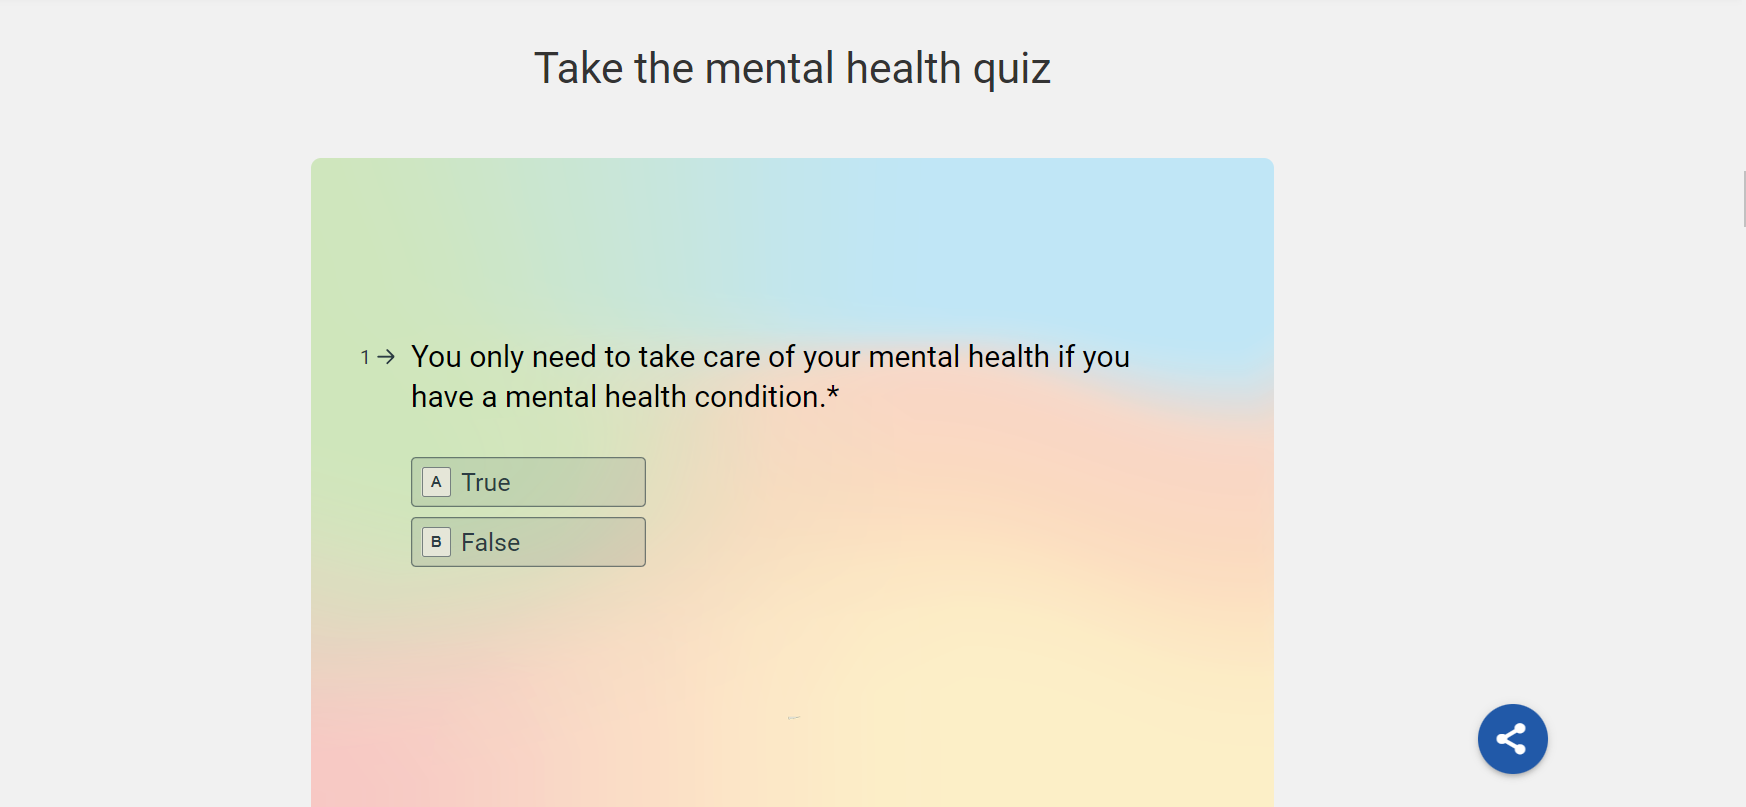
\includegraphics[width=\textwidth]{Picture12.png}
	\end{center}
	\captionsetup{font=small}
	\caption{\textit{Quiz example.}}
	\label{fig:label12}
\end{figure}

\paragraph*{H9. Help Users Recognize, Diagnose and Recover from Error  - Score 4}
Mistakes when filling forms are correctly highlighted, they are expressed in plain language (no error codes), precisely indicate the problem, and constructively suggest a solution. However, they are only reported after clicking “Submit”.

\begin{figure}[h]
	\centering
	\begin{center}
		
\includegraphics[width=\textwidth]{Picture13.png}
	\end{center}
	\captionsetup{font=small}
	\caption{\textit{Mistakes example.}}
	\label{fig:label13}
\end{figure}

\paragraph*{H10. Help and Documentation  - Score 2}
Help and documentation resources are present on the website, but not so easily accessible and mainly present in the form of text so difficult to read through due to the wall of text. The documentation lacks essentiality and concreteness. It is not present a chat to directly get in touch with UNICEF.

\newpage

\paragraph*{H11. Information Overload  - Score 2}
Across the whole website, often the information is too much resulting in difficulties in achieving tasks, due to the lack of conciseness. In some cases, information is correctly divided by colors/sections.
For example, in the page \href{https://www.unicef.org/early-childhood-development}{Early Childhood Development} the text is long, with poor hierarchy and there are present many different types of information (textual, visual such as cards, link, resources) that may confuse the user while searching for key information.

\paragraph*{H12. Consistency of Page Content Structure  - Score 1}
In general, the structure is not respected in the pages that present the same topics. For example, across the pages in the “Focus Areas” section we can find two different main organizations and even in the same organization structure, the pages present some minor inconsistencies in how elements are presented, implying a higher cognitive load.
For example, in some pages "Focus Areas" is present, while in some other pages it is not. The same is valid for the navigable index.
The pages \href{https://www.unicef.org/child-protection}{Child Protection} and \href{https://www.unicef.org/nutrition}{Nutrion}, despite being in the same section, present completely different elements in terms of visual aspect, as well as contents organization.

\paragraph*{H13. Contextualized Information  - Score 2}
In some pages, breadcrumbs are present, and this can help users in understanding where they are, as well as having a title for each page. Still, there are inconsistencies between the title of the page and the name present in the menu and the main section is not highlighted, making the user feels lost in the complexity of contents.
For example, if we open the page \href{https://www.unicef.org/gender-equality}{Gender}, we will read the title "Gender equality", as well as not seeing the section in the main menu highlighted. This inconsistency can lead to confusion and to easily get lost within the website.

\paragraph*{H14. Content Organisation (Hierarchy)  - Score 1}
The hierarchy of the contents does not respect the topic relevance, as every element present the same font size, hardly distinguished by bold or italic. The sections that organize the contents in each page seems to be random, without highlighting the most important to information to guide the user.
In the page \href{https://www.unicef.org/stories}{Stories} all the elements are presented with the same relevance, making the user feel lost with too many options.
In the page \href{https://www.unicef.org/gender-equality}{Gender} Data and Insights links have the same relevance as the Overview part.

\begin{figure}[h]
	\centering
	\begin{center}
		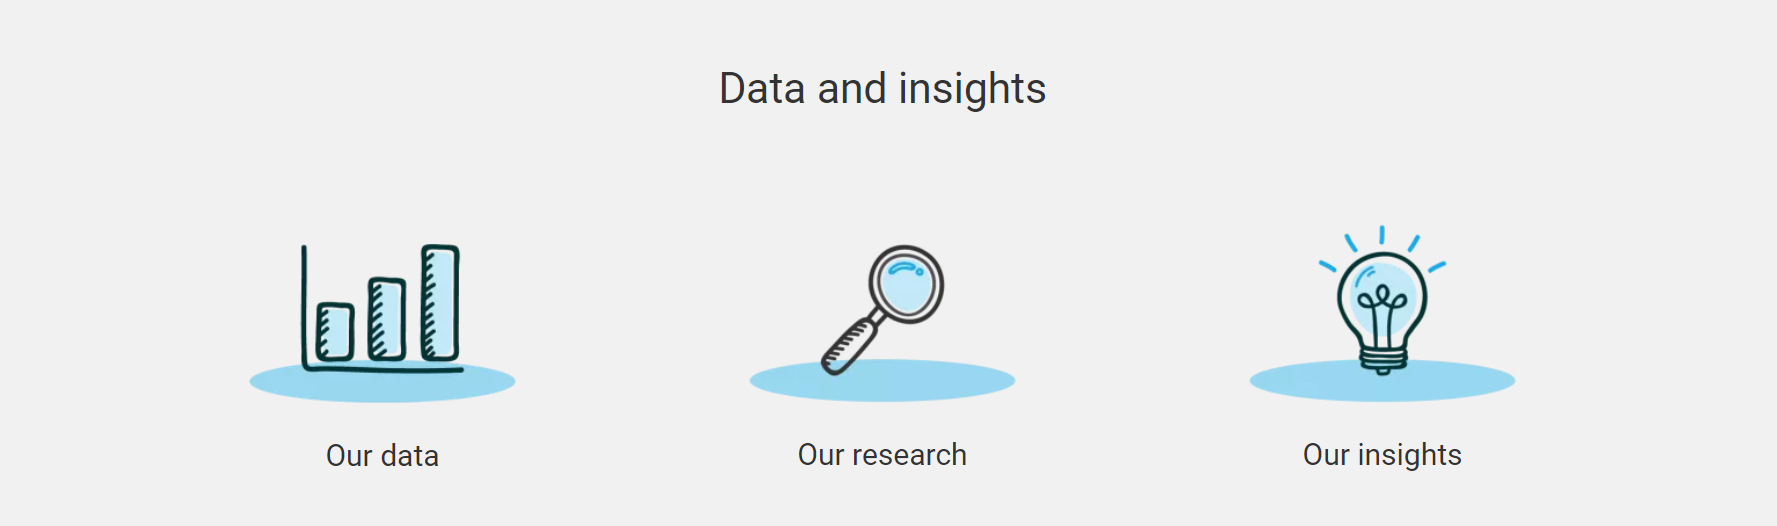
\includegraphics[width=0.6\textwidth]{Picture17.png}
	\end{center}
	\captionsetup{font=small}
	\caption{\textit{Data and Insights links.}}
	\label{fig:label17}
\end{figure}

Another example is the one of cards: they do not present hierarchy between the different types of contents. In fact, Reports or Blog Posts have the same relevance and the user can not understand which content to prioritize.

\begin{figure}[h]
	\centering
	\begin{center}
		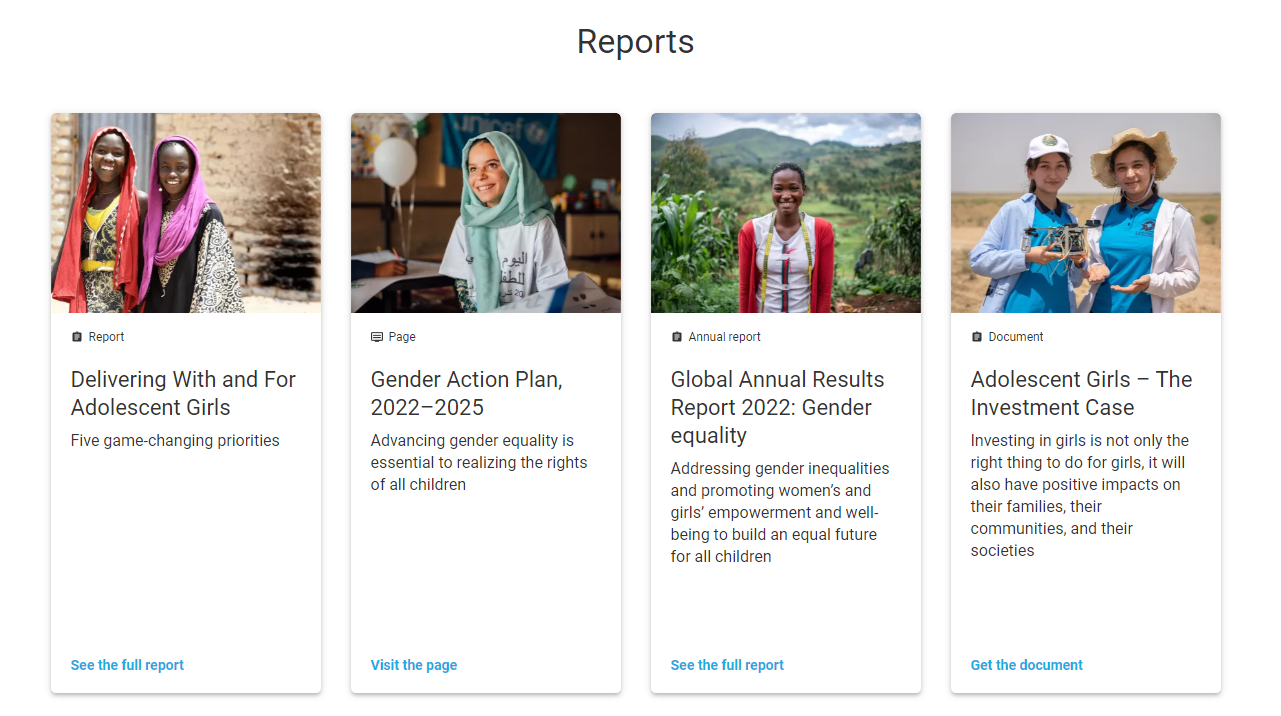
\includegraphics[width=0.8\textwidth]{Picture18.png}
	\end{center}
	\captionsetup{font=small}
	\caption{\textit{Reports cards.}}
	\label{fig:label18}
\end{figure}

\begin{figure}[h]
	\centering
	\begin{center}
		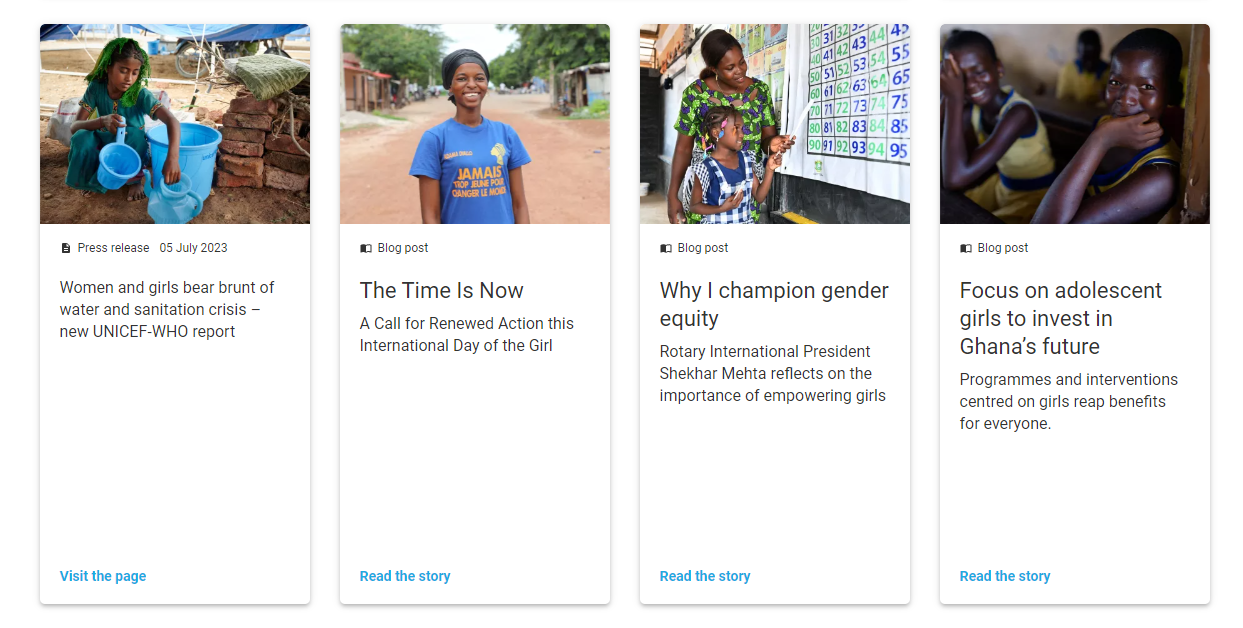
\includegraphics[width=0.8\textwidth]{Picture19.png}
	\end{center}
	\captionsetup{font=small}
	\caption{\textit{Blog Posts cards.}}
	\label{fig:label19}
\end{figure}

\paragraph*{H15. Interaction Consistency  - Score 3}
In general, pages of the same type have the same navigation links and capabilities, depending on the type of content presented. However, there are some inconsistencies that can affect the overall understanding of the website's patterns.

\paragraph*{H16. Group Navigation 1  - Score 2}
When breadcrumbs are present, the process of navigatin fro, among and within items is quite easy, but in the majority of the website these are not present. Moreover, when redirected to other specific websites, going back to UNICEF Global is not easy as the text button is small and hidden at the top of the page. This process results difficult due to the complexity of the hierarchy of the website and the lack of information about the position of the user. Moreover, when scrolling the page, the logo at the top doesn’t stay fixed so the Homepage is not accessible.

\paragraph*{H17. Group Navigation 2  - Score 3}
The main menu is quite simple and clear, with the section clearly differentiated with consistent names that matches the real world with an appropriate font size. However, when it comes to the pages in the drop-down menu, there are some inconsistencies such as “All areas” redirecting to “What we do” pages or names being presented differently when opening the page. These discrepancies may create cognitive load. Moreover, the amount of pages and information may confuse the user, so it would be useful to reorganise the information architecture of the website.

\begin{figure}[h]
	\centering
	\begin{center}
		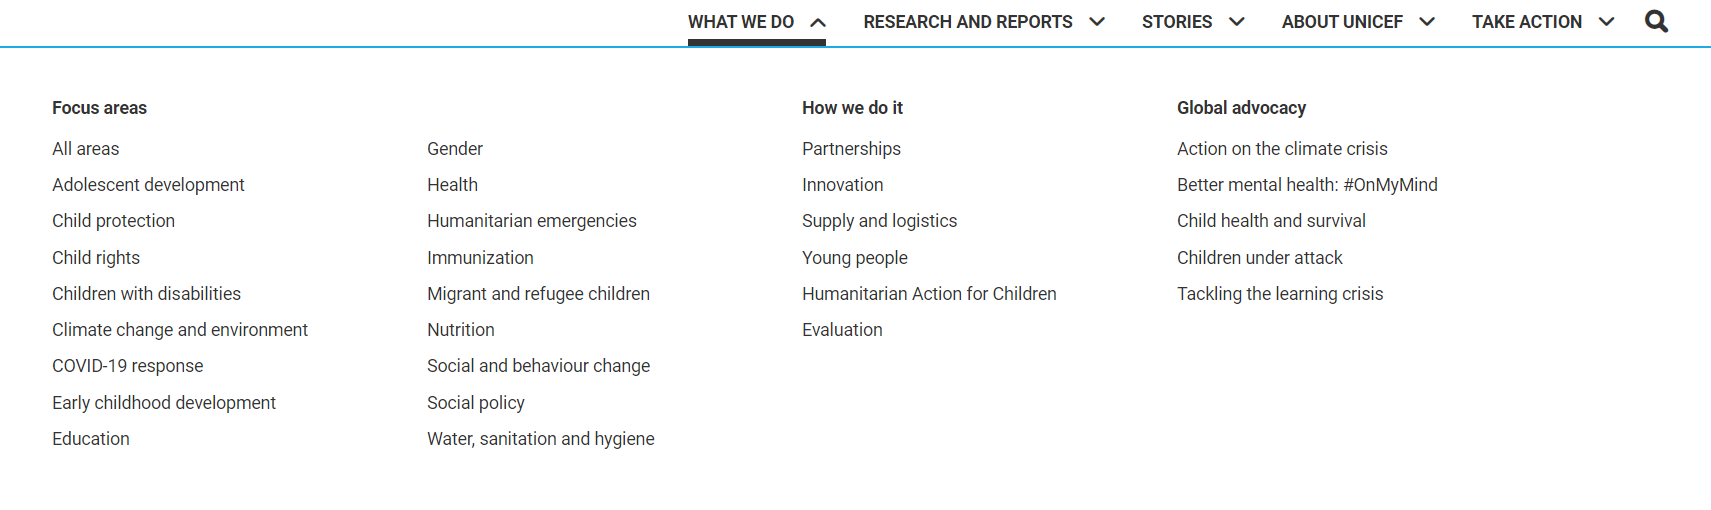
\includegraphics[width=\textwidth]{Picture20.png}
	\end{center}
	\captionsetup{font=small}
	\caption{\textit{Pages in the main menu.}}
	\label{fig:label20}
\end{figure}

\paragraph*{H18. Structural Navigation  - Score 3}
It is sufficiently easy to navigate among the components of a topic in terms of content accessibility, but the poor hierarchy makes it hard to understand which parts to prioritize.
One key example is the page of the report \href{https://www.unicef.org/reports/state-worlds-children-2023}{The State of the World’s Children 2023}, that presents many different types of contents, as well as not highlighting the most relevant ones. this may lead the user to feel lost and not in control.

\paragraph*{H19. Semantic Navigation  - Score 3}
Due to the lack of breadcrumbs in many parts of the website, the navigation from a topic to a related one is not so easy, as the user is often not informed about his/her position on the website. Moreover, the orientation clues are missing, such as highlighting the section of the main menu. Many types of documents exist (blog post, report, document, page) and they are not divided into section but presented all together, so understanding the relationship between contents is not easy.

\paragraph*{H20. Landmarks  - Score 3}
n general landmarks provide a fast access to the most relevant part of the website, both in the header and in the footer. However, some aspects should be improved to improve the overall easiness of navigation.
The homepage is accessible from all the pages, but the logo is not fixed so the scrolling is required to go back to the top of the page. Both the footer and the main menu provides access to the main sections of the website, even though the “Contact us” text button is too small to be visible and easily accessible. The “donate” button is always accessible and present in many different pages (core of the association), but its lack of consistency involves a higher cognitive load.

\paragraph*{H21. Text Layout  - Score 3}
The font size is appropriate in some parts of the website, while in others it is not. The body should be smaller to give a better visual hierarchy in the pages and make the reading easier. There should be a higher balance between titles, body text and links in some cases, as it is right now it does not correctly convey the hierarchy of contents.

\begin{figure}[h]
	\centering
	\begin{center}
		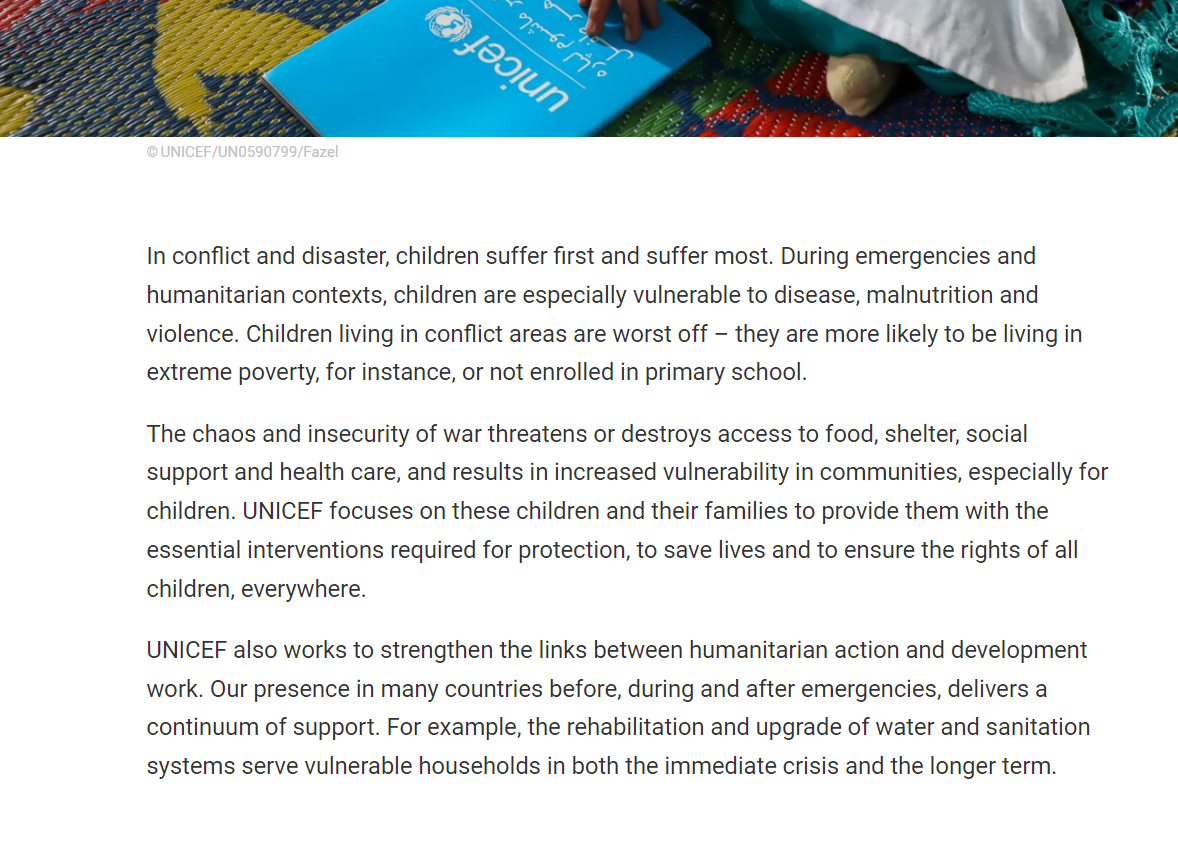
\includegraphics[width=0.6\textwidth]{Picture21.png}
	\end{center}
	\captionsetup{font=small}
	\caption{\textit{Huge body text.}}
	\label{fig:label21}
\end{figure}

\begin{figure}[h]
	\centering
	\begin{center}
		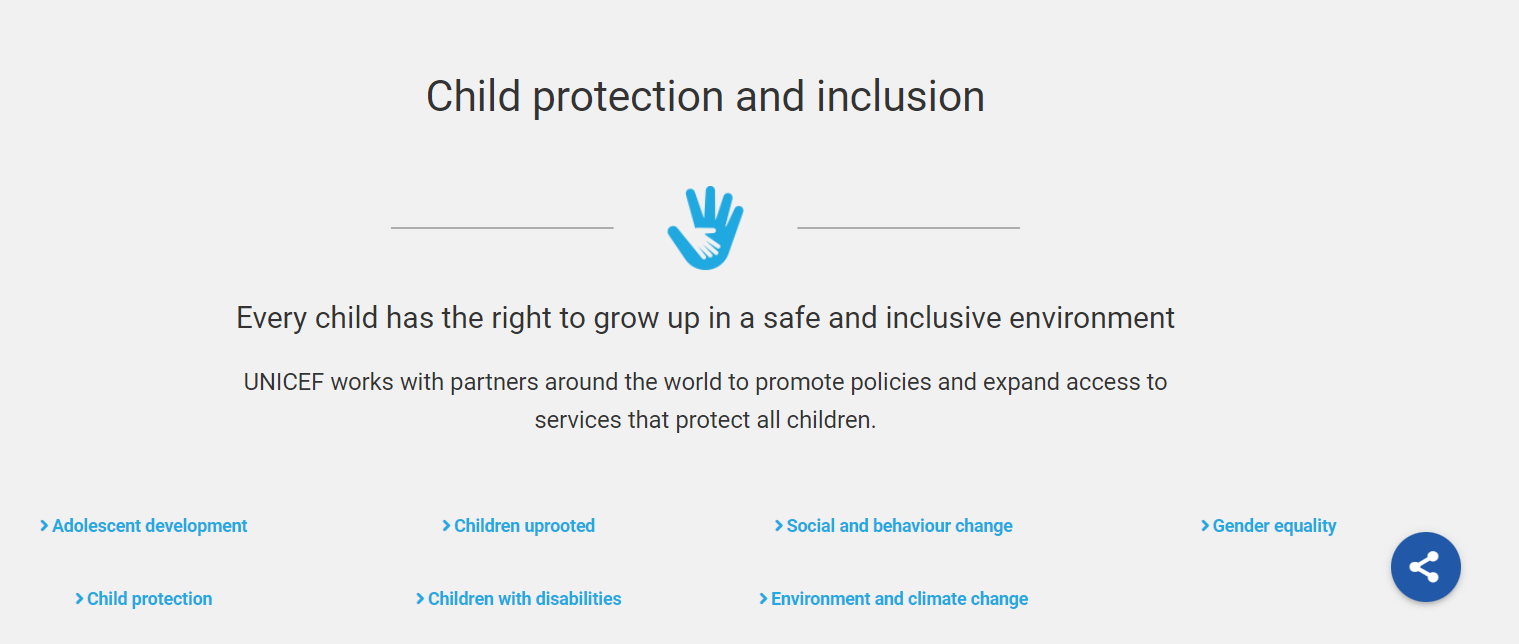
\includegraphics[width=0.6\textwidth]{Picture22.png}
	\end{center}
	\captionsetup{font=small}
	\caption{\textit{Hierarchy between title, body text and links.}}
	\label{fig:label21}
\end{figure}

\paragraph*{H22. Interaction Placeholders - Semiotics  - Score 3}
In general, interactive elements can be defined “intuitive”: links are coloured and underlined when overlaying with the mouse; clickable cards have an overlay shadow, as well as textual and primary buttons. 

\begin{figure}[h]
	\centering
	\begin{center}
		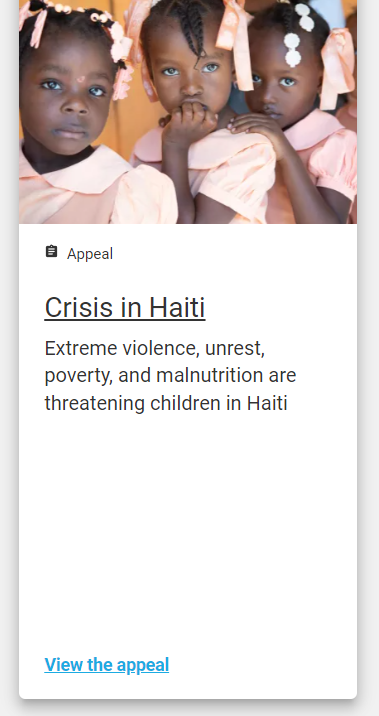
\includegraphics[width=0.1\textwidth]{Picture24.png}
	\end{center}
	\captionsetup{font=small}
	\caption{\textit{Card shadow.}}
	\label{fig:label23}
\end{figure}

There are some situations, however, in which it is difficult to understand whether an element is interactive or not, for example in the icons present in the section "Data and Insights". However, this does not compromise the overall usability.

\begin{figure}[h]
	\centering
	\begin{center}
		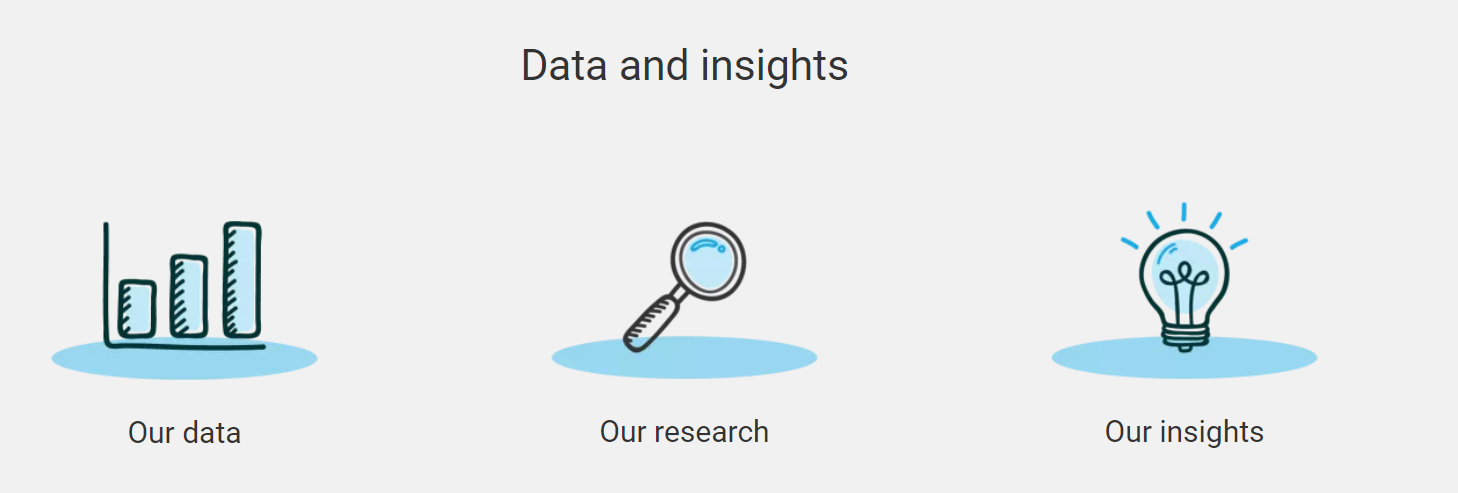
\includegraphics[width=0.6\textwidth]{Picture23.png}
	\end{center}
	\captionsetup{font=small}
	\caption{\textit{Clickable icons.}}
	\label{fig:label23}
\end{figure}

\newpage

\paragraph*{H23. Interaction Placeholders - Consistency  - Score 2}
Cards are consistent in the organization of contents, but follow a strange pattern of colour (white, blue, black), while buttons totally lack consistency. Buttons are a crucial aspect of usability, and their inconsistency can compromise the navigation.
Icons are generally consistent across the website, apart from minor exceptions.

\begin{figure}[h]
	\centering
	\begin{center}
		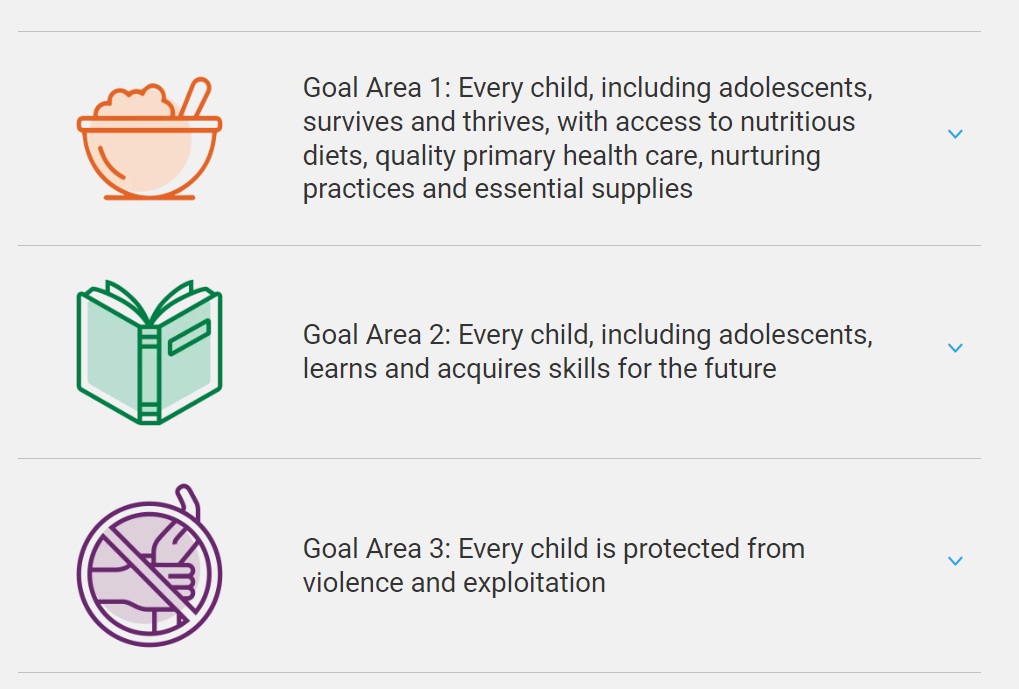
\includegraphics[width=0.6\textwidth]{Picture25.png}
	\end{center}
	\captionsetup{font=small}
	\caption{\textit{This kind of icons can be found only once.}}
	\label{fig:label23}
\end{figure}

\paragraph*{H24. Consistency of Visual Elements  - Score 2}
In pages of the same type, visual elements generally don’t have the same visual properties, and this create confusion in the user that can get lost in the page without catching the core information.
In the section "Emergencies Spotlight" all the pages present different visual elements that, however, convey the same information. For example, there are very differents call to action for finding out more about a topic (links, buttons).

\begin{figure}[h]
	\centering
	\begin{center}
		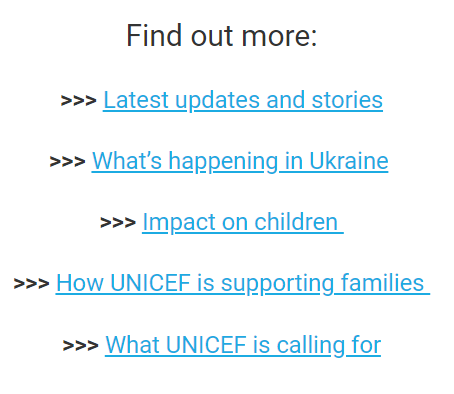
\includegraphics[width=0.3\textwidth]{Picture27.png}
	\end{center}
	\captionsetup{font=small}
	\caption{\textit{Call to action 1.}}
	\label{fig:label23}
\end{figure}

\begin{figure}[h]
	\centering
	\begin{center}
		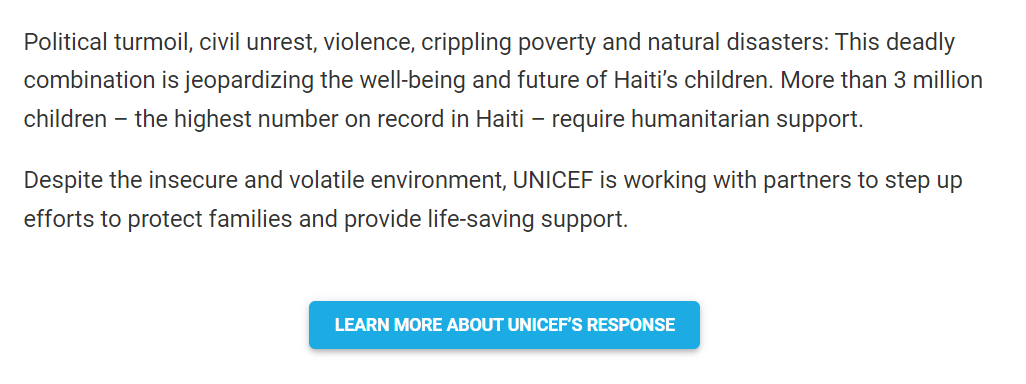
\includegraphics[width=0.6\textwidth]{Picture28.png}
	\end{center}
	\captionsetup{font=small}
	\caption{\textit{Call to action 2.}}
	\label{fig:label23}
\end{figure}

\newpage

At the same time, also the buttons for donating are very different and this inconsistency present across the whole website can generate insecurity towards which action to perform. 

\begin{figure}[h]
	\centering
	\begin{center}
		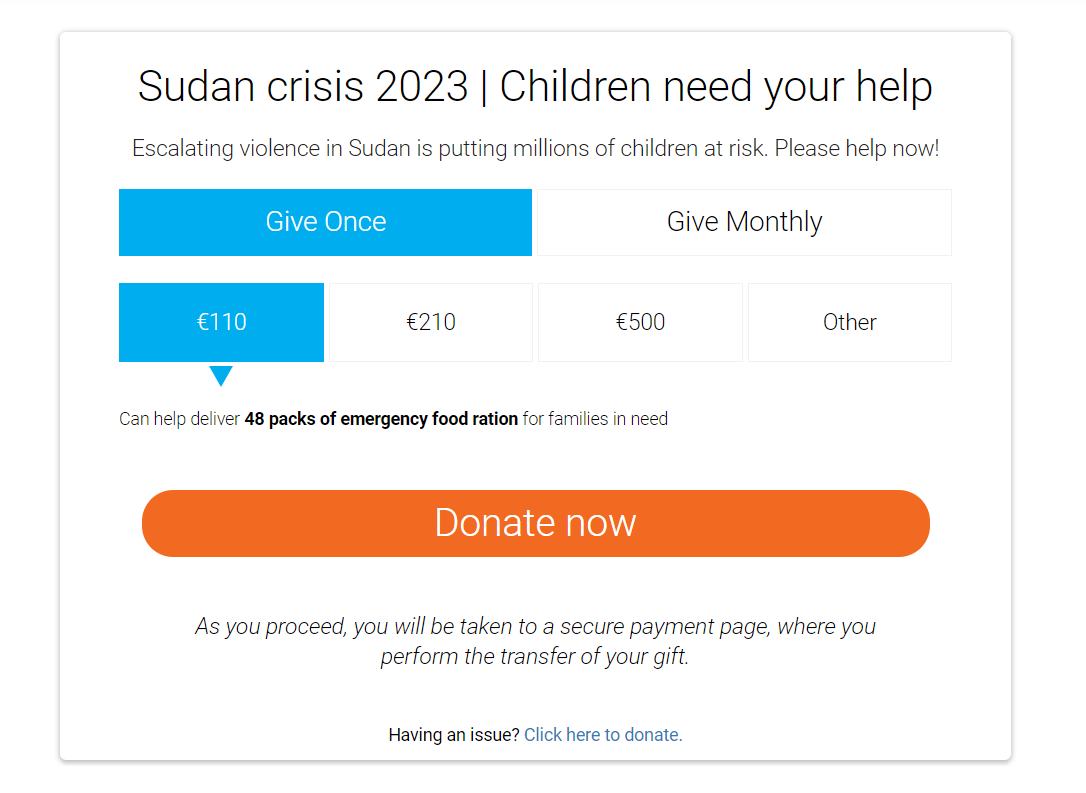
\includegraphics[width=0.4\textwidth]{Picture29.png}
	\end{center}
	\captionsetup{font=small}
	\caption{\textit{Donate button 1.}}
	\label{fig:label23}
\end{figure}

\begin{figure}[h]
	\centering
	\begin{center}
		
\includegraphics[width=0.6\textwidth]{Picture29B.png}
	\end{center}
	\captionsetup{font=small}
	\caption{\textit{Donate button 2.}}
	\label{fig:label23}
\end{figure}

\newpage

\paragraph*{H25. Hierarchy 1  - Score 2}
The on-screen allocation of contents somehow reflects their relevance, having an organization that follows the structure of giving at first a general introduction and then going deeper in what UNICEF is doing for the cause. However, the lack of hierarchy makes it difficult to prioritize even though the organization follows a meaningful order.
The \href{https://www.unicef.org/about-unicef}{Who we are} page reflects the lack of hierarchy in terms of font size and contents disposition, bombarding the user with an overload of information.

\paragraph*{H26. Hierarchy 2  - Score 1}
The on-screen allocation of visual elements does not reflect their relevance, as all the contents are basically the same size and occupy the whole screen, being at the centre of the page. In this way, it is difficult to prioritize and give attention to the most important piece of information.

\paragraph*{H27. Spatial Allocation 1  - Score 4}
Generally, semantically related elements are close to each other. For example, titles, body text and images that are connected are usually presented in a cohesive way.

\begin{figure}[h]
	\centering
	\begin{center}
		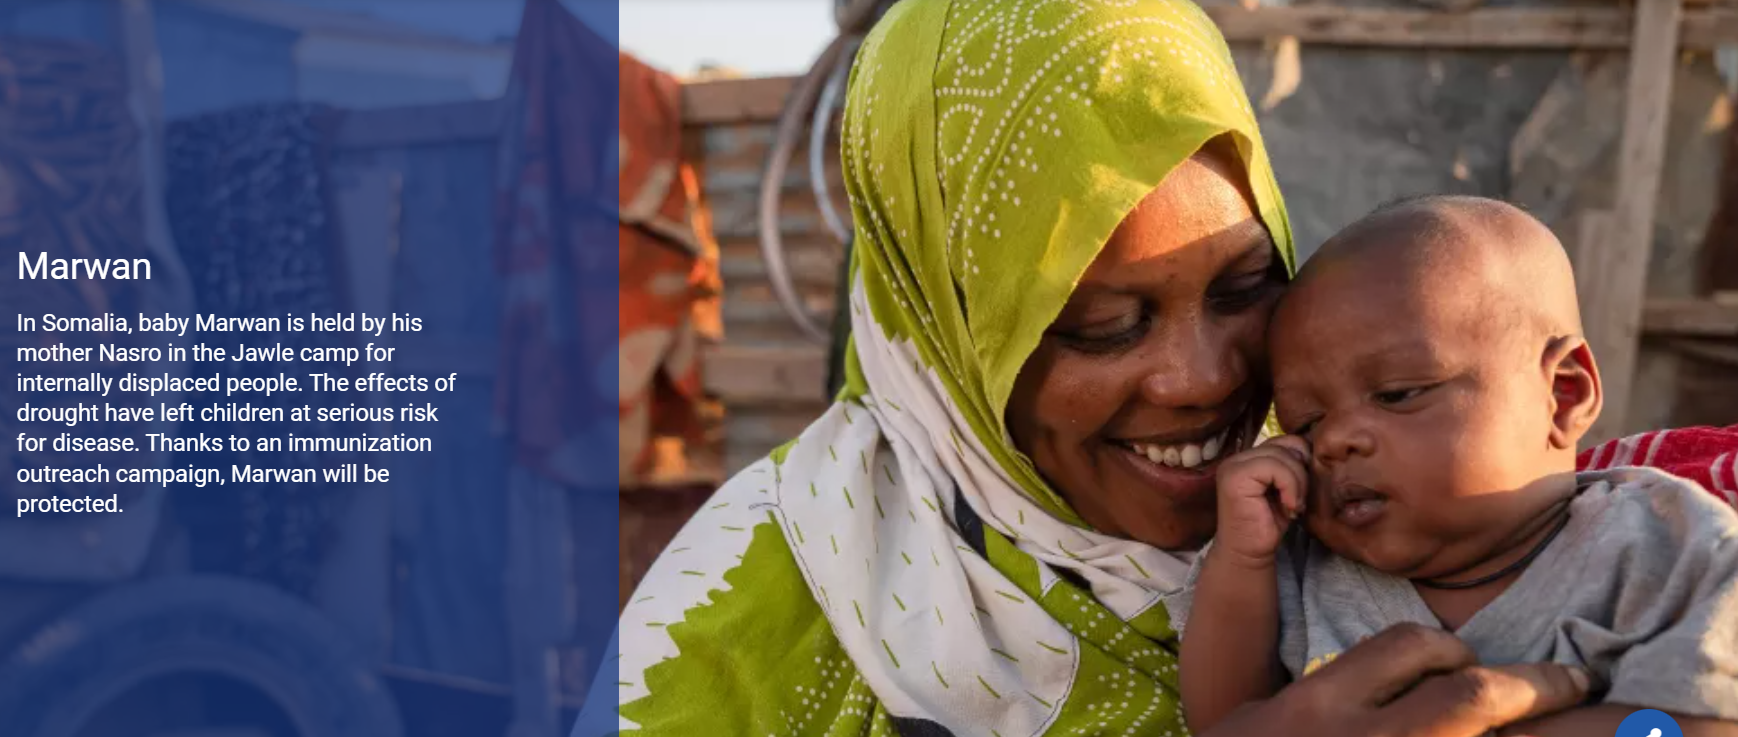
\includegraphics[width=\textwidth]{Picture30.png}
	\end{center}
	\captionsetup{font=small}
	\caption{\textit{Good semantic relationship.}}
	\label{fig:label23}
\end{figure}

\newpage

\paragraph*{H28. Spatial Allocation 2  - Score 3}
Semantically distant elements are usually divided with section of different colours (grey), but the body font size makes it hard to distinguish between each section.

\begin{figure}[h]
	\centering
	\begin{center}
		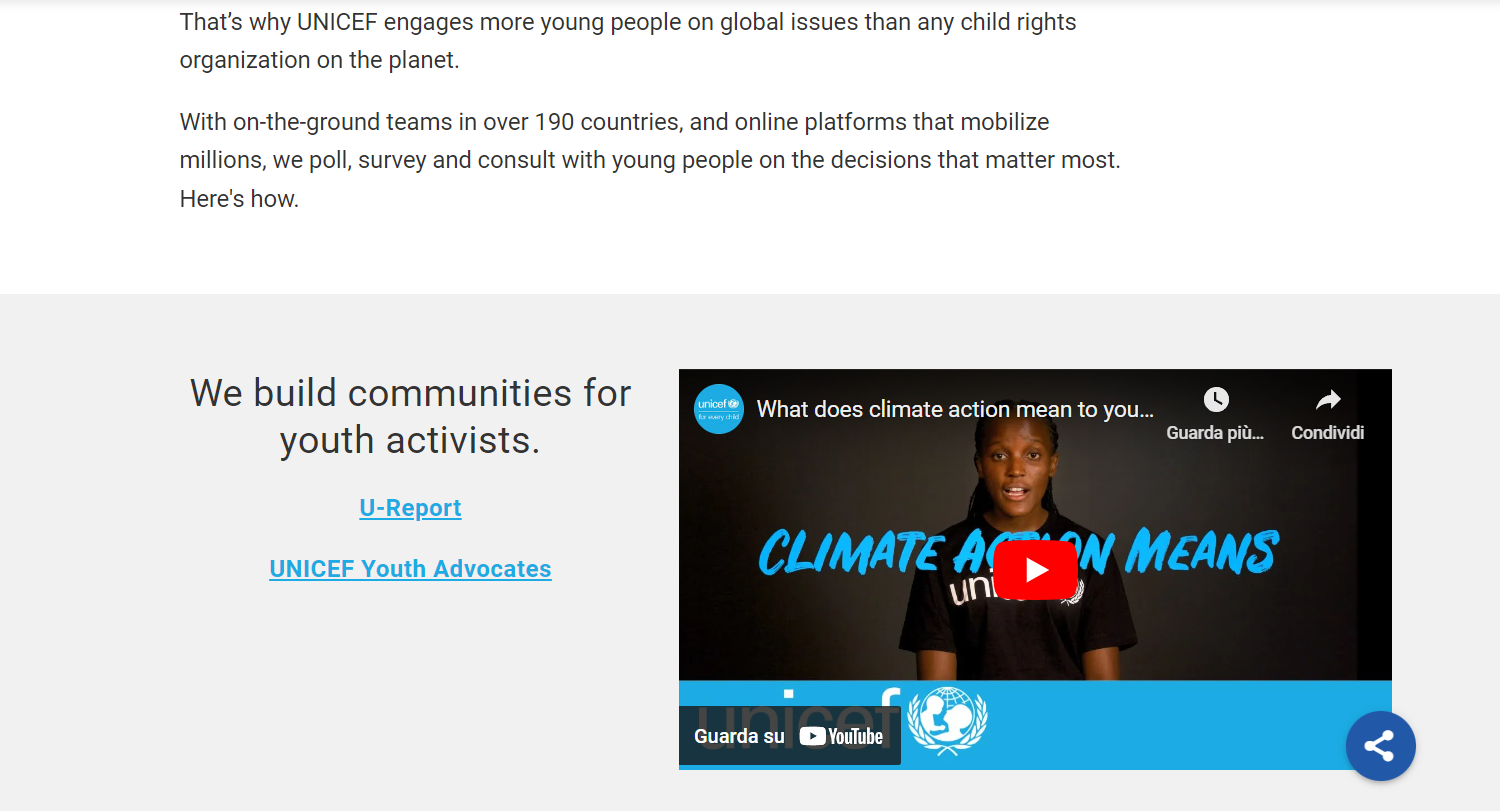
\includegraphics[width=\textwidth]{Picture31.png}
	\end{center}
	\captionsetup{font=small}
	\caption{\textit{Section with different colours.}}
	\label{fig:label23}
\end{figure}

\paragraph*{H29. Consistency of Page Spatial Structure  - Score 3}
Generally, pages of the same type have the same spatial organisation for the various visual elements. However, being the website overall quite inconsistent there are different exceptions, for example within the pages in the "Global Advocacy" section.